\subsection{Förbättringsförslag som resultat av intervjuer}\label{subsec:sfera-utokat}
Genom att studera SFERA-protokollets datauppsättning (avsnitt~\ref{subsec:dokumentanalys}) och lokförarnas kommunikations- och informationsbehov (~\ref{subsec:dokumentanalys}) har de kunnat jämföras med varandra.
De överlapp som finns argumenterar för att dessa delar från lokförarnas behov täcks upp av SFERA\@.
För de delar i intervjuerna som uppdagats rörande lokförarnas nämnda behov men som inte täcks av SFERA har ett utökningsförslag av SFERA tagits fram.
En illustration av detta ges i figur~\ref{fig:sferabehov}.
\begin{figure}[hbt!]
    \centering
    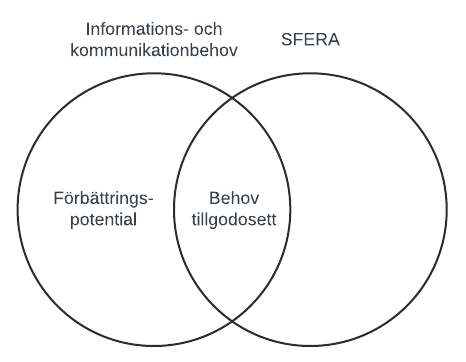
\includegraphics[width=0.5\textwidth]
    {sferabehov}
    \caption{Venndiagram som illustrerar förbättringspotential utifrån jämförelsen mellan datainsamlingsresultat och SFERA:s datauppsättning. Egen framställning.}
    \label{fig:sferabehov}
\end{figure}
\subsubsection{Kommunikation från TMS till C-DAS-OB}
Följande förbättringsförslag ges som går utöver SFERA-protokollet för kommunikation från tågklarerare till lokförare.
\paragraph{Journey profile}
Ett JP består idag av train characteristics (data om fordon), en lista över segment profile:r (data om aktuell(a) bana/banors egenskaper) samt avgångs- och ankomsttider för dessa, tillfälliga begränsningar (för exempelvis pådrag).
För att bättre möta lokförarnas behov inkluderas utöver nämn data försenings- eller omplaneringsorsak(er), avsändare av JP - vilken bandel och driftledningscentral meddelandet kommer från samt telefonnummer till denne.
Försenings- och omplaneringsinformation eller -orsak(er) efterfrågas uttryckligen av flera förare under intervjusessioner.
Att exempelvis veta var ett tåg ska gå om ett annat eller gå in på sidan på en driftplats för att släppa förbi ett tåg är ett gynnsamt sätt att bygga förtroende sett till respondenternas utsagor.
Rent tekniskt kan meddelandet läggas som en del av journey package så att denna information medföljer varje gång ny JP skickas ut.
Förbättringsförslaget illustreras i tabell~\ref{tab:jpImproved} och den nya datastrukturen illustreras i tabell~\ref{tab:omplanering}.
\begin{table}[hbt!]
    \centering
    \begin{tabular}{|l|}
        \hline
        \textbf{Journey profile} \\
        \hline
        - Unikt ID för berörd tågfärd \\
        - Tidskorridor \\
        - Train characteristics \\
        - Segment profile (lista av) \\
        - Dynamisk data \\
        \color{blue}
        - Omplaneringsorsak \\
        \hline
    \end{tabular}
    \caption{Datastruktur, journey profile (förbättringsförslag). Tillägg markerat med blå text.}
    \label{tab:jpImproved}
\end{table}
\begin{table}[hbt!]
    \centering
    \begin{tabular}{|l|}
        \hline
        \textbf{Omplaneringsorsak} \\
        \hline
        - Unikt ID för omplaneringsorsak \\
        - Orsak \\
        - Telefonnummer till avsändare \\
        - Avsändares bandel \\
        - Avsändares trafikledningscentral \\
        \hline
    \end{tabular}
    \caption{Datastruktur, omplaneringskontext samt kontaktuppgifter till avsändare.}
    \label{tab:omplanering}
\end{table}
\paragraph{Blankettförberedelse}
Före muntlig ordergivning måste blanketter förberedas som lokföraren är ålagd att medtaga under tågfärd.
Ordergivning genom diktamen sker genom att lokföraren upprepar vad tågklareraren säger samtidigt som denne noterar på en blankett vilken information som tas emot.
Om tågklareraren enkelt kan uppmana en eller fler lokförare i ett område att förbereda en specifik blankett för ordergivning kan många korta samtal potentiellt sett sparas in.
Därför läggs en typ av meddelanden till i SFERA-protokollet som ska skickas från TMS via TS-servrar till C-DAS-OB när en fjärrtågklarerare vill uppmana lokförare att förbereda en specifik blankett.
Idag finns inget lämpligt meddelande som blankettförberedelse kan rymmas inom då all kommunikation från TMS till C-DAS-OB sker genom JP\@, och JP skickas ut endast vid omplanering av tidtabell.
Detta innebär att en ny meddelandetyp tas fram som kallas \emph{train message}, varuti blankettförberedelse kan rymmas.
\paragraph{Kontaktuppgifter}
Att veta vilket telefonnummer som går till aktuellt driftledningsområde kan vara fördelaktigt att ha lättillgängligt.
I synnerhet vid körning utomlands där det kan vara svårare att snabbt hitta rätt information.
Därför kompletteras datauppsättningen för segment profile med telefonnummer till aktuell bandels tågklarerare.
\paragraph{Trafikstörningar}
Idag kan information om trafikstörningar gå en lång omväg från en driftledningscentral innan den når lokföraren.
Om lokföraren får information direkt från ursprungskällan med plats, tid, påverkan och prognos för trafikstörningar kan information istället ges snabbt till kunder.
Ett TMS många tåg inom ett avgränsat område.
Denna funktionalitet införs därför som en ny form av meddelande.
Trafikstörningar kan läggas till i segment profile för en aktuellt geografisk punkt.
\begin{table}
    \centering
    \begin{tabular}{|l|l|l|}
        \hline
        \textbf{Segment profile} & & \\
        \hline
        - Unikt ID & & \\
        - Version & & \\
        - Längd & & \\
        \hline
        SP-punkter & SP-karaktäristik & SP-områden \\
        - Trafikplats & - Banans STH för ett visst segment & - Station, plattform \\
        - etc & - etc & - etc \\
        \color{blue}
        - Trafikstörningar & & \\
        \hline
    \end{tabular}
    \caption{Datastruktur, segment profile. För att se originalet i sin helhet, se tabell~\ref{tab:sp}.}
    \label{tab:spImproved}
\end{table}
\paragraph{Meddelande om uppdaterad tåglängd}
Enligt utsagor från intervjuobjekten kan tvära kast i fordonsplanering som innebär förändring av tåglängd förekomma, av flera olika skäl.
Det vore därför av intresse för förarna att kunna se vilken tåglängd tågklarerarna \emph{tror} att en viss tågfärd har.
Om detta visar sig inte överensstämma med verkligheten kan lokföraren kontakta tågklareraren med GMS-R-telefonsamtal och delge korrekt information.
Det framgår inte helt av analyserad dokumentation om lokförarna direkt kan skicka information om förändringar i tåglängd.
Informationen finns i TC, men om C-DAS-OB kan skicka förändringar i TC genom status report är inte helt tydligt.
Om så är fallet kan korrekt tåglängd delges direkt till TMS\@.
\begin{table}[hbt!]
    \centering
    \begin{tabular}{|l|}
        \hline
        \color{blue}
        \textbf{TMS message} \\
        \hline
        - Unikt ID för berörd tågfärd \\
        - Uppmaning, blankettförberedelse (blankettnummer) \\
        - Aktuell tåglängd \\
        - Avsändares trafikledningscentral \\
        \hline
    \end{tabular}
    \caption{Datastruktur, blankettförberedelse eller återgivelse av inrapporterad tåglängd.}
    \label{tab:tmsMessage}
\end{table}
%\paragraph{Context awareness}
%GPS-position av tåg tillhandahålls TMS som därför borde kunna återge en grupp av kringliggande tågs GPS-position för ett särskilt tåg.
%Att öka lokförarnas situationsmedvetenhet har pekats ut både i litteraturstudie och intervjuer som en viktig informationspunkt.
%Därför kompletteras SFERA med information från TMS till C-DAS-OB om GPS-positioner av tåg i ett enskilt tågs omgivning.
\subsubsection{Kommunikation från C-DAS-OB till TMS}
Följande förbättringsförslag ges som går utöver SFERA-protokollet för kommunikation från lokförare till tågklarerare.
\paragraph{Kvittens av JP}
När ett JP skickas ut bör det göras tydligt för föraren att ny tidtabell är aktuell.
Denna kan då bekräftas eller avvisas om föraren uppenbart märker att tågklarerarens plan inte kommer att kunna realiseras i praktiken.
\paragraph{Rapportering av balisinformationsfel}
När balisinformationsfel\footnote{Baliser är signalsystemets gränssnitt för informationsöverföring från signalsystem till tågets hastighetsövervakningssystem. De tar emot information banutrustningen och strömsätts när ett tåg passerar dem, varpå information kan överföras till tågen. Om information tåget emottager inte är fullständig \lq{}vet inte\rq{} längre tågets skyddssystem vilken information som gäller och kommer begränsa tågets STH till 80 km/h eller 40 km/h beroende på var tåget befinner sig, och lokföraren måste köra under restriktioner\cite{TTJ2015}.} inträffar ska lokföraren delge tågklarerare om var det inträffat, vilka konsekvenser som gavs samt vilken felkod som presenterades.
Förarna uppgav i intervjuer att det kan vara svårt att veta exakt var det inträffade och vilken balisgrupp som avses.
En del förare uppgav också att de och deras kollegor ibland slarvar med att rapportera in balisinformationsfel till driftledningscentralen.
Längden STH begränsas kan vara upp till 3800 m \emph{plus} tågsättets längd, vilket skulle kunna innebära måttlig påverkan en tågfärds rättidighetsförmåga.
Om lokföraren inte rapporterat detta till driftledningscentralen kan tågklareraren fatta beslut baserat på felaktigt informationsunderlag.
För att underlätta för både lokförare och tågklarerare införs därför ett meddelande där lokföraren kan skicka GPS-position, ja/nej för driftbroms och släcka indikatorer samt felkod.
Tågklareraren kan då snabbt få reda på att ett tågs STH begränsas, frekvensen av inrapportering kan öka och inrapportering kan bli en enklare process för lokföraren.
\begin{table}[hbt!]
    \centering
    \begin{tabular}{|l|l|}
        \hline
        \color{blue}
        \textbf{Balisinformationsfel} \\
        \hline
        - Balisinformationsfel typ 1 & bool  \\
        - Driftbroms och 80- eller 40-övervakning & bool \\
        - Felkod & sträng \\
        - GPS-position & sträng \\
        \hline
    \end{tabular}
    \caption{Datastruktur, inrapportering av balisinformationsfel.}
    \label{tab:bf}
\end{table}
\paragraph{Plattformsbehov}
För persontåg kan det vara aktuellt med särskilt behov av plattform vid antingen höger eller vänster sida av tåget.
Det kan röra sig om ett större antal avstängda in- och avstigningsdörrar på ena sidan eller om en dörr är avstängd vid en handikapplift.
Om detta på enkelt vis kan meddelas i god tid till tågklareraren kan det leda till snabbare trafikutbyte.
\begin{table}[hbt!]
    \centering
    \begin{tabular}{|l|}
        \hline
        \color{blue}
        \textbf{Plattformsbehov} \\
        \hline
        - Höger eller vänster \\
        - Tid (minuter) \\
        \hline
    \end{tabular}
    \caption{Datastruktur, äskande om särskild sida för trafikutbyte eller extra plattformstid.}
    \label{tab:plattformsbehov}
\end{table}
\paragraph{Meddelande om plötsligt stopp}
Ibland uppstår fordonsfel som kan leda till att ett tåg gör ett oplanerat stopp.
Det händer enligt respondenterna att driftledningscentralen inte svarar direkt när man ringer, och om man har ett akut fordonsfel kan det vara stressande att vänta på att någon svarar.
En funktion som meddelar driftledningscentralen att ett tåg har fått ett stoppande fel är sannolikt av intresse för en tågklarerare då de skulle kunna delges information att ett tåg står still även om de är upptagna med andra uppgifter.
Det skulle möjliggöra att en lokförare snabbt kan meddela tågklarerare att tåget står still, eventuell prognos och sedan direkt påbörja felsökning och åtgärd utan att först behöva ringa och delge information muntligen.
Information kan kompletteras i efterhand via GSM-R-samtal.
\paragraph{Meddelande om signal i stopp}
Under intervjuerna framgick det att förarna var av åsikten att bra järnvägstrafik var konsekvensen av ett bra samspel mellan lokförare och tågklarerare.
Det fanns en förståelse för att båda parter är människor och ibland gör fel.
Att tågklarerare ibland glömmer bort tåg för en kort period föreföll oundvikligt, och då kunde det hända att tåg blir ståendes vid röda signaler som visar stopp.
Då kunde förarna känna sig påträngande eller onödigt ivriga vid samtal i dessa lägen då orsaken kanske var enkel eller kortvarig.
Om förarna å andra sidan avstod från att ringa i dessa lägen kanske det skulle leda till att de stod i dessa lägen onödigt länge ifall tågklareraren faktiskt glömde bort tåget.
Ett meddelande med en notis om att ett tåg håller för stopp vid en viss signal införs därför.
Meddelandet kan besvaras med mottagningsbekräftelse med eventuell orsak och prognos vid händelser av lägre dignitet såsom korsande tågväg.
\paragraph{Meddelande till SOS}
Från en respondent som suttit i samrådsmöten med räddningstjänst, ambulans och polis framgick det att den här typen av samhällsfunktioner har svårt att identifiera exakt position för tåg de ska undsätta, i synnerhet för poliser.
Är det tågstopp kan många tåg befinna sig nära varandra vilket kan försvåra lokalisering.
Därför föreslås en funktion där C-DAS-OB kan delge GPS-position till SOS Alarm direkt eller via IM DAS-TS\@.
I dagsläget passeras informationen i många led muntligen från lokförare till operativ blåljuspersonal med flera led emellan vilket potentiellt kan leda till att information tappas på vägen.
Det har enligt respondenten visat sig hänt flera gånger i verkligheten samtidigt som nämnda samhällsfunktioner efterfrågan denna typ av funktionalitet.
Detta förslag går eventuellt lite långt ifrån ämnet, men oavsett är det tågklarerarna som kontaktar SOS Alarm och om systemet möjliggör distribution av GPS-information skulle det potentiellt kunna vara av intresse för polis, ambulans och räddningstjänst.
\paragraph{Meddelande om att samtal önskas}
Det framgick under intervjuerna att lokförare ibland behöver kontakta tågklarerare, men i ärenden som inte är akuta.
När de då ringer driftledningscentralen i dessa ärenden kan det ibland gå så lång tid att föraren väljer att lägga på och istället försöka senare.
Respondenten tillade att detta inte är något konstigt i sig, utan att tågklareraren förmodligen är upptagen.
Att då kunna skicka ett meddelande om att samtal önskas kan avlasta tågklarerarens uppmärksamhet.
\paragraph{Reducerad dragkraft}
Information om dragkraft görs tillgängligt för TMS via RU DAS-TS men C-DAS-OB förefaller inte ha någon möjlighet att skicka detta direkt till TMS i status report.
Därför läggs denna meddelandetyp till och består av en andelsangivelse i förhållande till den fulla potential som finns i fordon enligt train characteristics.
